\documentclass[tikz,border=2pt]{standalone}
\usepackage{amsmath}
\usetikzlibrary{arrows.meta}
\begin{document}
% Binary rating factors A, B with interaction under a log link: the rate ratio for A is
% e^{beta_A} = 1.2 when B = 0 and e^{beta_A + beta_AB} = 1.2 x 1.5 = 1.8 when B = 1.
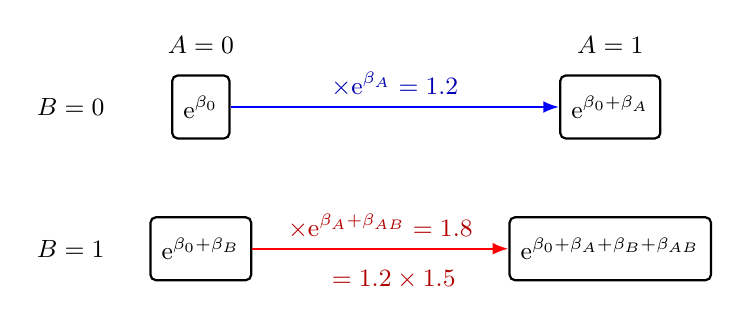
\begin{tikzpicture}[font=\small, >={Latex[length=2mm]},
    cell/.style={draw, thick, rounded corners=2pt, minimum height=0.8cm, inner sep=4pt}]
  \node[anchor=south] at (0,0.55) {$A=0$};
  \node[anchor=south] at (5.2,0.55) {$A=1$};
  \node[anchor=east] at (-1.1,0) {$B=0$};
  \node[anchor=east] at (-1.1,-1.8) {$B=1$};
  \node[cell] (a) at (0,0) {$\mathrm{e}^{\beta_0}$};
  \node[cell] (b) at (5.2,0) {$\mathrm{e}^{\beta_0+\beta_A}$};
  \node[cell] (c) at (0,-1.8) {$\mathrm{e}^{\beta_0+\beta_B}$};
  \node[cell] (d) at (5.2,-1.8) {$\mathrm{e}^{\beta_0+\beta_A+\beta_B+\beta_{AB}}$};
  \draw[->, thick, blue] (a) -- node[above, blue!70!black] {$\times \mathrm{e}^{\beta_A}=1.2$} (b);
  \draw[->, thick, red] (c) -- node[above, red!70!black] {$\times \mathrm{e}^{\beta_A+\beta_{AB}}=1.8$} (d);
  \node[red!70!black, anchor=north] at (2.45,-1.95) {$=1.2\times1.5$};
\end{tikzpicture}
\end{document}
